\documentclass{article}
\usepackage{bookmark}

\usepackage[utf8]{inputenc}
\usepackage[brazil]{babel}  % Define o idioma para português do Brasil
\usepackage{csquotes}       % Para lidar com aspas de maneira apropriada com babel
\usepackage{array}
\usepackage{amsmath}
\usepackage{xcolor}

\usepackage{amsmath}
\usepackage{xcolor}
\usepackage{listings}
% Configuração do estilo de código
\lstset{
  language=C,
  %basicstyle=\ttfamily\footnotesize,
  keywordstyle=\color{blue},
  commentstyle=\color{gray},
  stringstyle=\color{red},
  breaklines=true,
  frame=single,
  numbers=left,
  numberstyle=\tiny,
  numbersep=5pt,
  showstringspaces=false,
}


\usepackage{graphicx}       % Pacote para inserção de imagens

\usepackage{hyperref}       % Pacote para links clicáveis
\hypersetup{
    colorlinks=true,
    linkcolor=blue,
    urlcolor=blue,
}

\usepackage{enumitem}       % Pacote para personalização de listas

\usepackage{geometry}       % Pacote para ajustar margens

\geometry{                  % Definindo margens personalizadas (em centímetros)
  left=2.5cm,  % Margem esquerda
  right=2.5cm, % Margem direita
  top=2.5cm,   % Margem superior
  bottom=2.5cm % Margem inferior
}

\usepackage[backend=biber,style=ieee]{biblatex}     % Estilo ieee para bibliografia numerada
\addbibresource{ref.bib}                            % Arquivo .bib


\begin{document}

\begin{titlepage}
    \centering
    % Cabeçalho personalizado
    
\includegraphics[width=0.3\textwidth]{../../Topic1/Avaliativo/Imagens/Logo UFLA - Colorida chapada.png}

    \vspace*{2cm} % Espaçamento vertical antes do cabeçalho
    \Large
    Universidade Federal de Lavras\\
    PPGCC\\
    PCC508 – Sistemas Operacionais\\
    
    \vspace{2cm} % Espaço entre o cabeçalho e o título
    \huge % Define o tamanho da fonte do título
    \textbf{Tópico 6 Lista Avaliativa}
    
    \vfill % Adiciona um espaçamento flexível antes do rodapé (opcional)
    
    % Opcionalmente, você pode incluir seu nome e a data aqui
    \large
    Douglas Aquino T. Mendes\\
    \today % Insere a data atual
\end{titlepage}

\tableofcontents
\newpage

\section{Introdução}
Este documento tem como objetivo apresentar o desenvolvimento das atividades avaliativas para o tópico 6 da disciplina de Sistemas Operacionais, focando na implementação de códigos em linguagem C. Serão apresentadas as questões, a resolução, os códigos desenvolvidos, seguidos de uma explicação sobre sua lógica de funcionamento.

\section{Questões}

\subsection{Questão 1}
\textbf{Pergunta:} 1) Explique como nomes longos de arquivos podem ser manipulados em diretórios\newline

\textbf{Resposta:} Uma opção é manter os nomes dos arquivos em um heap no final de cada diretório. Cada entrada do diretório contém então um ponteiro para o nome do arquivo no heap. Essa abordagem evita a fragmentação e garante que uma nova entrada de arquivo sempre caiba no diretório. No entanto, o heap precisa ser gerenciado e podem ocorrer falhas de página ao processar nomes de arquivos \parencite[p. 145]{tanenbaum2021}. 

\subsection{Questão 2}

\textbf{Pergunta:} 2) Como funciona o Journaling em um sistema de arquivos? Explique.\newline

\textbf{Resposta:} O journaling em um sistema de arquivos é uma técnica que aumenta a \textit{``robustez"} do sistema diante de falhas, como quedas de energia ou travamentos. A ideia central é registrar as operações que serão realizadas no sistema de arquivos em um diário (journal) antes de executá-las \parencite[p. 145]{tanenbaum2021}.

\begin{itemize}
  \item As operações de escrita são primeiramente registradas no diário. 
  \item O diário é escrito no disco e verificado para garantir a integridade da escrita.
  \item Somente após a confirmação da escrita no diário, as operações de escrita no sistema de arquivos são executadas.
  \item Após a conclusão bem-sucedida das operações, a entrada correspondente no diário é apagada.
  \item Se ocorrer uma falha durante esse processo, o sistema de arquivos, ao ser reiniciado, consulta o diário para identificar as operações pendentes. As operações pendentes são então reexecutadas até que sejam concluídas com sucesso.
  \item Para garantir o funcionamento adequado do journaling, as operações registradas no diário devem ser idempotentes, o que significa que podem ser repetidas múltiplas vezes sem causar efeitos colaterais negativos. 
\end{itemize}


\subsection{Questão 3}

\textbf{Pergunta:} 3) Explique como funciona a alocação de blocos de arquivos baseadas em Inodes.  \newline

\textbf{Resposta: } Funcionamento da alocação de blocos baseada em inodes:
\begin{itemize}
  \item Criação do Inode: Quando um arquivo é criado, o sistema de arquivos aloca um inode (abreviação de "index node" é uma estrutura de dados que contém informações sobre um arquivo) para ele e armazena os atributos do arquivo no inode.
  \item Alocação de Blocos: O inode contém uma lista de endereços de blocos de disco. Inicialmente, essa lista pode estar vazia. Conforme o arquivo cresce e os dados são gravados, o sistema de arquivos aloca blocos de disco para o arquivo e adiciona seus endereços à lista no inode.
  \item Acesso aos Dados: Quando um processo precisa acessar os dados do arquivo, o sistema de arquivos usa o nome do arquivo para localizar seu inode. Em seguida, o sistema de arquivos usa a lista de endereços de blocos no inode para acessar os blocos de disco que contêm os dados do arquivo.
\end{itemize}



\subsection{Questão 4}

\textbf{Pergunta:} 4) Explique como funciona uma tabela FAT (File Allocation Table). \newline

\textbf{Resposta:} A FAT funciona como uma tabela na memória principal, onde cada entrada corresponde a um bloco no disco. Cada entrada na tabela contém um ponteiro para o próximo bloco do arquivo, ou um marcador especial para indicar o fim do arquivo ou um bloco defeituoso \parencite[p. 196, 222]{tanenbaum2021}.
O funcionamento da FAT pode ser ilustrado da seguinte forma:

\begin{itemize}
  \item Criação de um Arquivo: Quando um arquivo é criado, o sistema de arquivos aloca o primeiro bloco disponível no disco e registra o número desse bloco na entrada do diretório do arquivo. A entrada na FAT correspondente ao bloco alocado aponta para um marcador especial, indicando o fim do arquivo.
  \item Escrita de Dados: Quando dados são escritos no arquivo, o sistema de arquivos aloca outro bloco livre e atualiza a entrada na FAT do bloco anterior para apontar para o novo bloco alocado. A entrada na FAT do novo bloco, por sua vez, aponta para o marcador de fim de arquivo.
  \item Leitura de Dados: Para ler os dados do arquivo, o sistema de arquivos começa na entrada do diretório do arquivo, que contém o número do primeiro bloco. O sistema consulta a FAT para obter o número do próximo bloco e continua seguindo a cadeia de ponteiros até o marcador de fim de arquivo.

\end{itemize}

\subsection{Questão 5}

\textbf{Pergunta:} 5) Quando uma aplicação necessita de um controle mais aprimorado sobre as permissões associadas a um determinado arquivo, as Access Control Lists (ACL) podem ser utilizadas para isso. Descrever uma visão geral de como as ACLs funcionam.\newline

\textbf{Resposta:} \begin{itemize}
  \item Uma ACL é composta por uma lista de ACEs. Cada ACE especifica um usuário ou grupo e as permissões concedidas ou negadas a eles para o arquivo em questão.
  \item As permissões podem incluir leitura, escrita, execução e outras ações específicas, como "anexar" para arquivos ou "listar conteúdo" para diretórios.
  \item As ACLs podem ser configuradas para herdar permissões de diretórios pai, simplificando a administração de permissões em estruturas hierárquicas de arquivos.
\end{itemize}

\textbf{Exemplo:} Imagine um arquivo confidencial de um projeto. Com as ACLs, é possível conceder permissões de leitura e escrita aos membros da equipe do projeto. Conceder permissão de leitura apenas para o gerente do projeto. Negar explicitamente o acesso a todos os outros usuários, independentemente de suas permissões de grupo.


\section{Desenvolver um programa}

\subsection{Enunciado 6}

\textbf{Enunciado:}  A chamada statvfs(…) é utilizada para obter-se informações sobre um sistema de arquivos montado. Faça um programa que receba como parâmetro o caminho de um sistema de arquivos e apresente as informações obtidas através desta chamada.\newline

\subsubsection{Código}
\label{sub-sec-cod1}
\lstinputlisting[language=C]{Codes/atv6.c}

\subsubsection{Testes e Resultados}
Como resultado da execução do código exibido na subceção \ref{sub-sec-cod1}, obtivemos a saída ilustrada na figura \ref{fig:exec1}. 

\begin{figure}[ht]
    \centering
    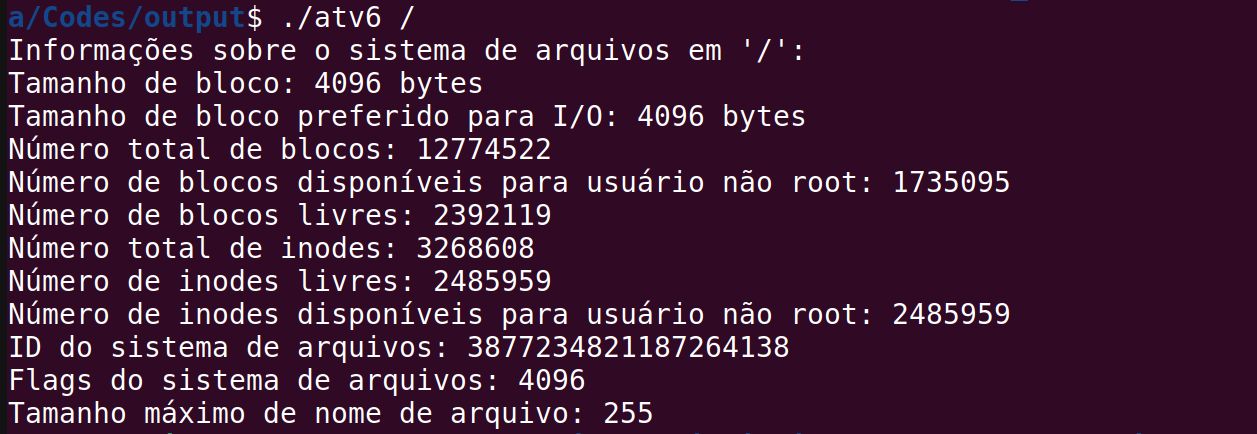
\includegraphics[width=1\textwidth]{./Images/res6.png}
    \caption{Resultado da execução do programa}
    \label{fig:exec1}
\end{figure}

\subsection{Enunciado 7}

\textbf{Enunciado:}   Criar dois programas. O primeiro cria um arquivo binário, com 30 ints, realizando uma contagem (1,2,3,4...30). Isso significa que os 30 ints devem ser armazenados em sequência no arquivo. O segundo programa deve utilizar a função readv para fazer a leitura simultânea em múltiplos buffers de 8 números do arquivo gerado pelo primeiro programa. Essa leitura deve ser feita somente com uma instrução readv. Os números a serem lidos devem ser a partir do décimo armazenado (décimo no buffer 1, décimo primeiro no buffer 2, e assim por diante). Imprimir os números na tela. Não esqueça que cada int tem o seu tamanho em bytes fixo.\newline

\subsubsection{Código}
\label{sub-sec-cod}
\lstinputlisting[language=C]{Codes/atv7cod1.c}
\lstinputlisting[language=C]{Codes/atv7cod2.c}


\subsubsection{Testes e Resultados}
Como resultado da execução do código exibido na subceção \ref{sub-sec-cod}, obtivemos a saída ilustrada na figura \ref{fig:exec}. Fica a observação de que não tenho certeza se entendi corretamente o que deveria ser implementado.

\begin{figure}[ht]
    \centering
    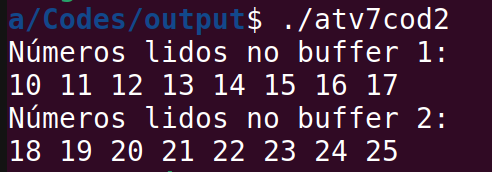
\includegraphics[width=1\textwidth]{./Images/res7.png}
    \caption{Resultado da execução do programa}
    \label{fig:exec}
\end{figure}

\printbibliography % Imprime a lista de referências


\end{document}